%%%%%%%%%%%%%%%%%%%%%%%%%%%%%%%%%%%%%%%%%
% Beamer Presentation
% LaTeX Template
% Version 1.0 (10/11/12)
%
% This template has been downloaded from:
% http://www.LaTeXTemplates.com
%
% License:
% CC BY-NC-SA 3.0 (http://creativecommons.org/licenses/by-nc-sa/3.0/)
%
%%%%%%%%%%%%%%%%%%%%%%%%%%%%%%%%%%%%%%%%%

%----------------------------------------------------------------------------------------
%	PACKAGES AND THEMES
%----------------------------------------------------------------------------------------

%\documentclass[UTF8,aspectratio=169,14pt]{ctexbeamer}
\documentclass[UTF8,aspectratio=169]{ctexbeamer}
\usepackage{hyperref}
\hypersetup{
	colorlinks=true,
	linkcolor=red,
	anchorcolor=blue,
	citecolor=green
}

\mode<presentation> {
	
	% The Beamer class comes with a number of default slide themes
	% which change the colors and layouts of slides. Below this is a list
	% of all the themes, uncomment each in turn to see what they look like.
	
	%\usetheme{default}
	%\usetheme{AnnArbor}
	%\usetheme{Antibes}
	%\usetheme{Bergen}
	%\usetheme{Berkeley}
	%\usetheme{Berlin}
	%\usetheme{Boadilla}
	%\usetheme{CambridgeUS}
	%\usetheme{Copenhagen}
	%\usetheme{Darmstadt}
	%\usetheme{Dresden}
	%\usetheme{Frankfurt}
	%\usetheme{Goettingen}
	%\usetheme{Hannover}
	%\usetheme{Ilmenau}
	%\usetheme{JuanLesPins}
	%\usetheme{Luebeck}
	\usetheme{Madrid}
	%\usetheme{Malmoe}
	%\usetheme{Marburg}
	%\usetheme{Montpellier}
	%\usetheme{PaloAlto}
	%\usetheme{Pittsburgh}
	%\usetheme{Rochester}
	%\usetheme{Singapore}
	%\usetheme{Szeged}
	%\usetheme{Warsaw}
	
	% As well as themes, the Beamer class has a number of color themes
	% for any slide theme. Uncomment each of these in turn to see how it
	% changes the colors of your current slide theme.
	
	%\usecolortheme{albatross}
	%\usecolortheme{beaver}
	%\usecolortheme{beetle}
	%\usecolortheme{crane}
	%\usecolortheme{dolphin}
	%\usecolortheme{dove}
	%\usecolortheme{fly}
	%\usecolortheme{lily}
	%\usecolortheme{orchid}
	%\usecolortheme{rose}
	%\usecolortheme{seagull}
	%\usecolortheme{seahorse}
	%\usecolortheme{whale}
	%\usecolortheme{wolverine}
	
	%\setbeamertemplate{footline} % To remove the footer line in all slides uncomment this line
	%\setbeamertemplate{footline}[page number] % To replace the footer line in all slides with a simple slide count uncomment this line
	
	%\setbeamertemplate{navigation symbols}{} % To remove the navigation symbols from the bottom of all slides uncomment this line
}

\usepackage{graphicx} % Allows including images
\graphicspath{{./figs/}}
\usepackage{booktabs} % Allows the use of \toprule, \midrule and \bottomrule in tables
\usepackage{longtable}
\usepackage{listings}
\usepackage{xcolor}
\lstset{numbers=left, %设置行号位置
	numberstyle=\tiny, %设置行号大小
	keywordstyle=\color{blue}, %设置关键字颜色
	commentstyle=\color[cmyk]{1,0,1,0}, %设置注释颜色
	frame=single, %设置边框格式
	escapeinside=``, %逃逸字符(1左面的键),用于显示中文
	%breaklines, %自动折行
	extendedchars=false, %解决代码跨页时,章节标题,页眉等汉字不显示的问题
	xleftmargin=2em,xrightmargin=2em, aboveskip=1em, %设置边距
	tabsize=4, %设置tab空格数
	showspaces=false %不显示空格
}
% Fonts
% \usepackage{libertine}
% \setmonofont{Courier}
\setCJKsansfont[ItalicFont=Noto Serif CJK SC Black, BoldFont=Noto Sans CJK SC Black]{Noto Sans CJK SC}
\setmainfont[Ligatures={Common,TeX}]{Linux  Libertine O}
\setmonofont[SmallCapsFont={Latin Modern Mono Caps}]{Latin Modern Mono Light}
\setsansfont{Linux Biolinum O}

\logo{
\includegraphics[width=0.55cm,height=0.55cm]{../../thcs-logo.png}}

%----------------------------------------------------------------------------------------
%	TITLE PAGE
%----------------------------------------------------------------------------------------

\title[第6讲]{第6讲 :The Programming Languages of OS} % The short title appears at the bottom of every slide, the full title is only on the title page
\subtitle{第三节:A Study of Bugs on Linux }
\author{陈渝} % Your name
\institute[清华大学] % Your institution as it will appear on the bottom of every slide, may be shorthand to save space    
{
	清华大学计算机系 \\ % Your institution for the title page
	\medskip
	\textit{yuchen@tsinghua.edu.cn} % Your email address
}
\date{\today} % Date, can be changed to a custom date


\begin{document}

\begin{frame}
\titlepage % Print the title page as the first slide
\end{frame}

%\begin{frame}
%\frametitle{提纲} % Table of contents slide, comment this block out to remove it
%\tableofcontents % Throughout your presentation, if you choose to use \section{} and \subsection{} commands, these will automatically be printed on this slide as an overview of your presentation
%\end{frame}
%
%%----------------------------------------------------------------------------------
%%	PRESENTATION SLIDES
%%----------------------------------------------------------------------------------------
%
%%------------------------------------------------
%\section{第一节:课程概述} % Sections can be created in order to organize your presentation into discrete blocks, all sections and subsections are automatically printed in the table of contents as an overview of the talk
%%------------------------------------------------

%-------------------------------------------------
\begin{frame}[plain]
	\frametitle{Introduction}
	
	
	
	\begin{columns}
		
		\begin{column}{.3\textwidth}
			
			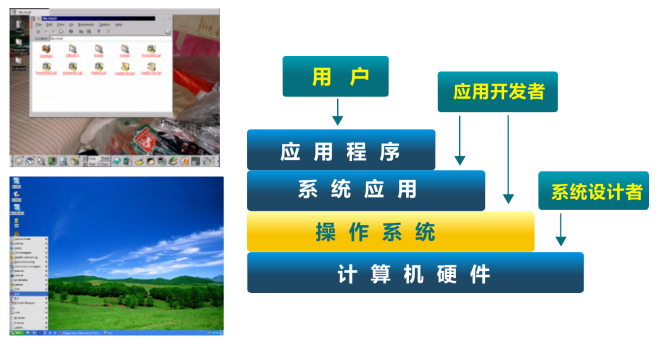
\includegraphics[width=1.\textwidth]{os-position}
			
		\end{column}
		
		\begin{column}{.7\textwidth}
			
			\Large
			Why study faults/bugs/Vulnerabilities in OS code?
			
			\begin{itemize}
				\item Find the relations between Language and OS
				
				
			\end{itemize}
			
		\end{column}
		
		
	\end{columns}
	
	
\end{frame}

%-------------------------------------------------
\begin{frame}[plain]
	\frametitle{Introduction}
	
	
	
	\begin{columns}
		
		\begin{column}{.3\textwidth}
			
			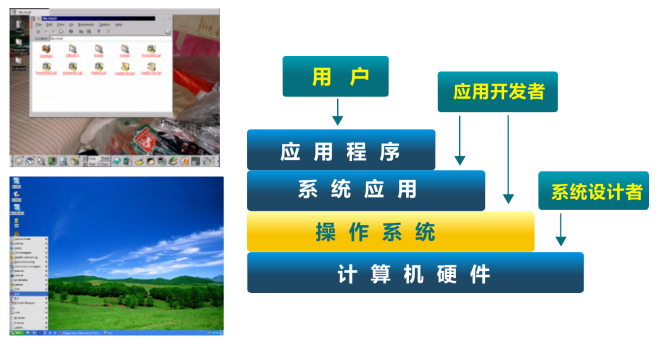
\includegraphics[width=1.\textwidth]{os-position}
			
		\end{column}
		
		\begin{column}{.7\textwidth}
			
			\Large
			Some questions
			\begin{itemize}
				\item  Where are the errors?
				
				\item How are bugs distributed?
				
				\item How long do bugs live?
							
			\end{itemize}
			
		\end{column}
		
		
	\end{columns}
	
	
\end{frame}


%-------------------------------------------------
\begin{frame}[plain]
	\frametitle{Introduction -- 19 years ago}
	
	
	
	\begin{columns}
		
		\begin{column}{.5\textwidth}
			
			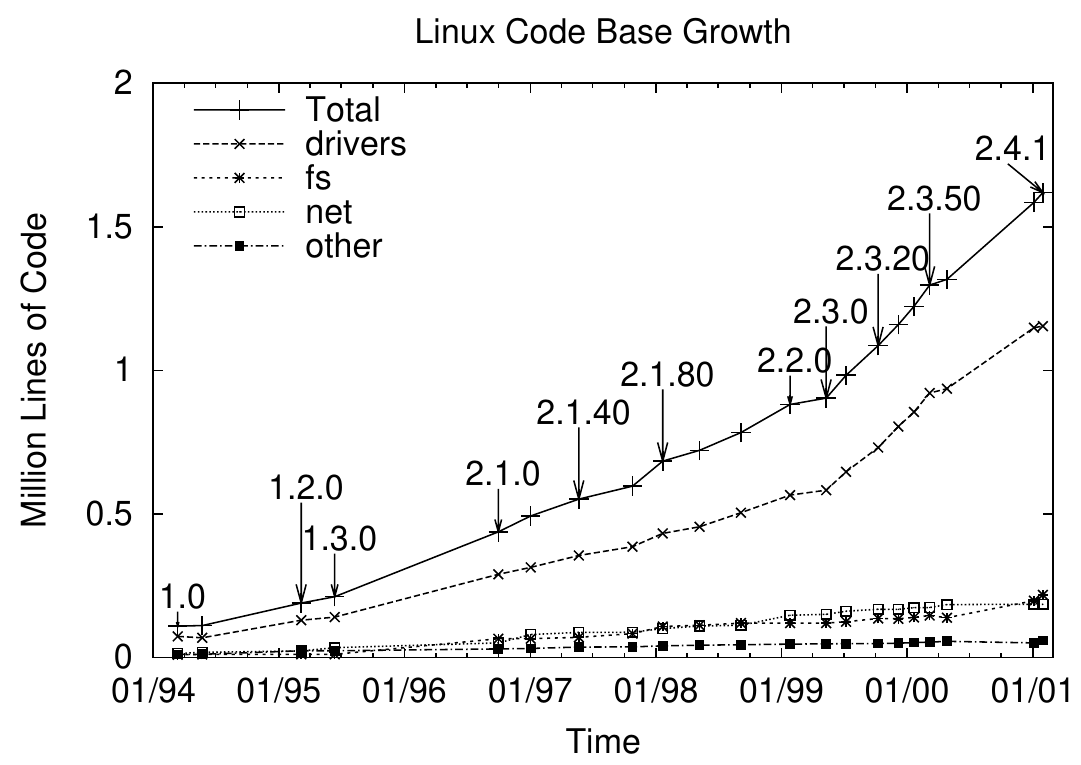
\includegraphics[width=1.\textwidth]{linux-code-sosp01}
			
		\end{column}
		
		\begin{column}{.5\textwidth}
			
%			\Large
			19 years ago
			
			\begin{itemize}
				\item   In SOSP'01, Chou et al. studied faults (errors/bugs) in Linux
				code.

				\item Faults collected using static analysis.
				
				
				\item Faults collected in Linux 1.0 (1994) to 2.4.1 (2001). Primarily “development” versions.  x86 code.
				
				
			\end{itemize}
			
		\end{column}
		
		
	\end{columns}
	
	
\end{frame}


%-------------------------------------------------
\begin{frame}[plain]
	\frametitle{Introduction -- 19 years ago}
	\centering
    The twelve  bug checkers
	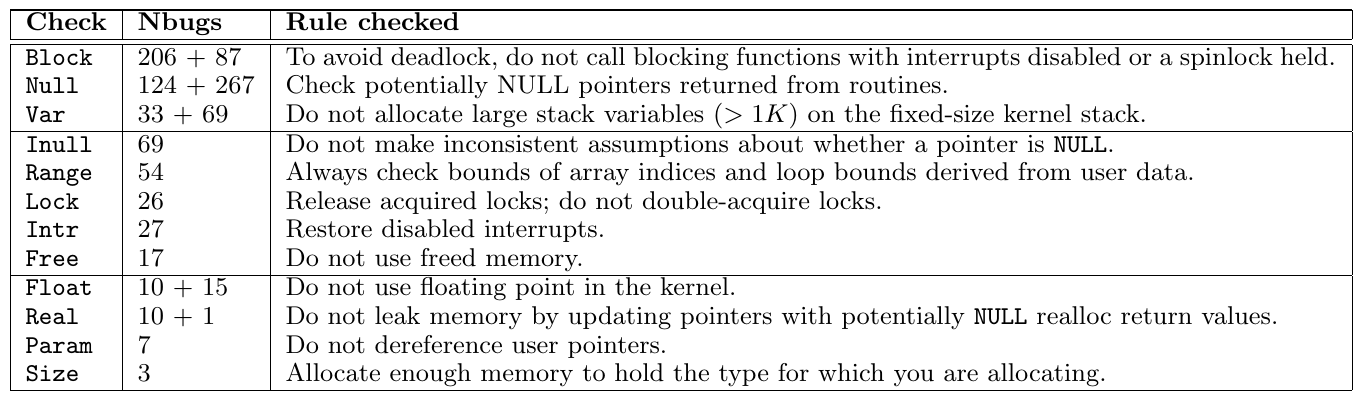
\includegraphics[width=1.\textwidth]{bug-check-sosp01}
	
\end{frame}



%-------------------------------------------------
\begin{frame}[plain]
	\frametitle{Introduction -- 19 years ago}
	
	
	
	\begin{columns}
		
		\begin{column}{.5\textwidth}
			
			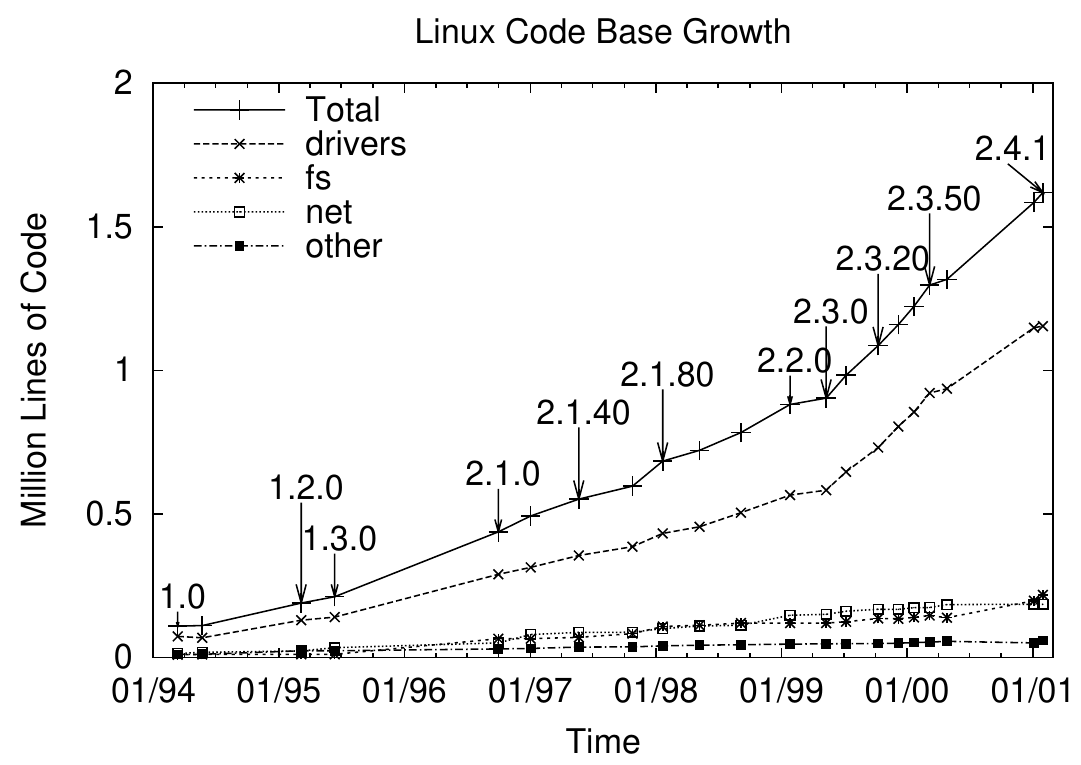
\includegraphics[width=1.\textwidth]{linux-code-sosp01}
			
		\end{column}
		
		\begin{column}{.5\textwidth}
			
			%			\Large
			Often condensed to the most important finding: “Drivers are
			the one major source of bugs in operating systems”, which
			becomes the scientific fundament for a huge body of OS
			research:
			
			
			\begin{itemize}
				\item Mike Swift: Nooks, Microdrivers ,	Carbon
				\item Tanenbaum: Minix 3
				\item UNSW: Dingo + Termite
				\item Gun Sirer: Reference Validation 
				\item Microsoft: Singularity + Signed Drivers 
				
				
			\end{itemize}
			
		\end{column}
		
		
	\end{columns}
	
	
\end{frame}


%-------------------------------------------------
\begin{frame}[plain]
	\frametitle{Introduction -- 19 years ago}
	\centering
	deadlock/data race related bug
     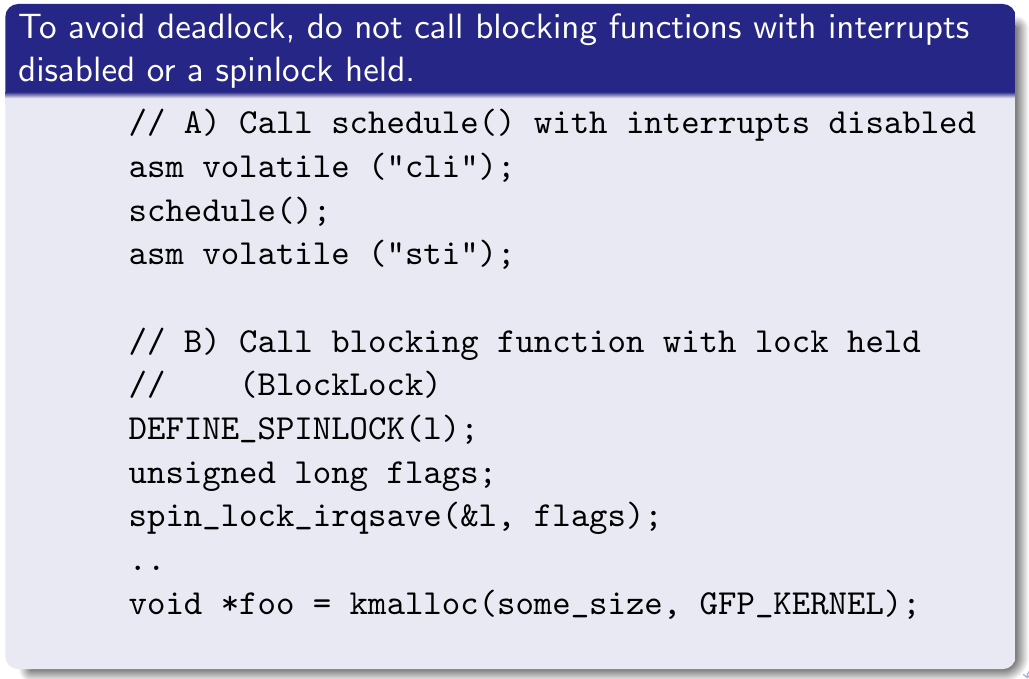
\includegraphics[width=.7\textwidth]{block-bug-sosp01}

\end{frame}

%-------------------------------------------------
\begin{frame}[plain]
	\frametitle{Introduction -- 19 years ago}
	\centering
	NULL/Free related bug
	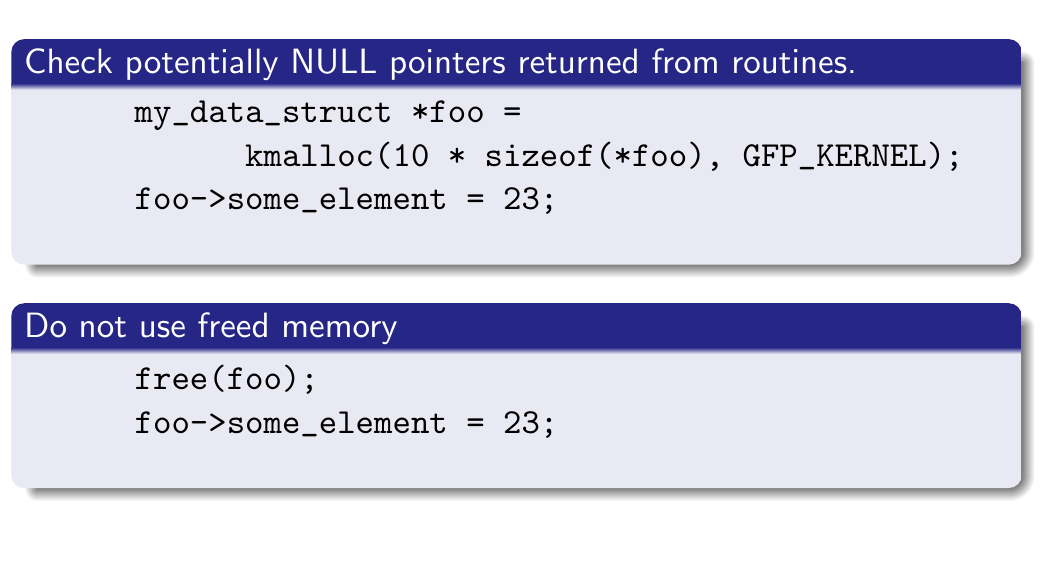
\includegraphics[width=.8\textwidth]{free-bug-sosp01}
	
\end{frame}


%-------------------------------------------------
\begin{frame}[plain]
	\frametitle{Introduction -- 19 years ago}
	\centering
	Var related bug
	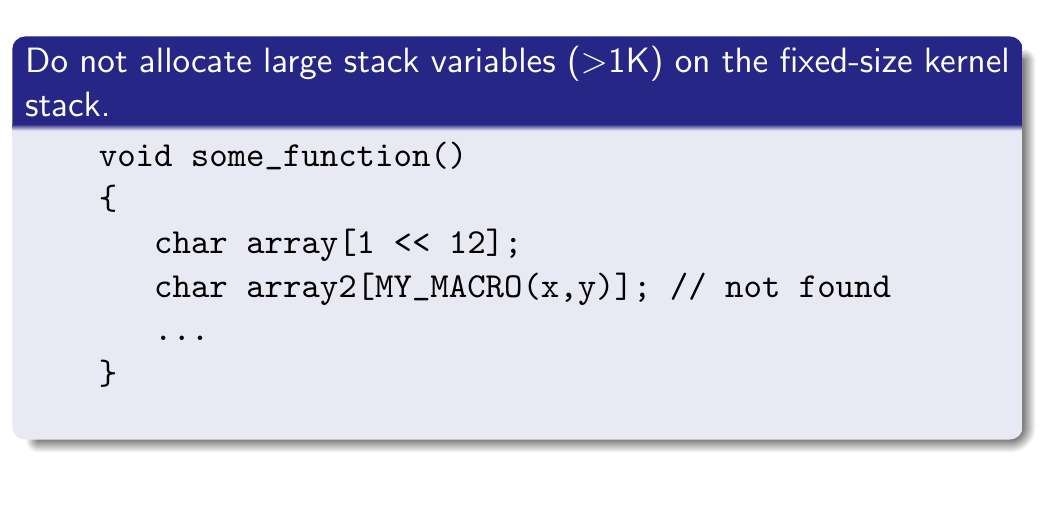
\includegraphics[width=.9\textwidth]{var-bug-sosp01}
	
\end{frame}

%-------------------------------------------------
\begin{frame}[plain]
	\frametitle{Introduction -- 19 years ago}
	\centering
	Range related bug
	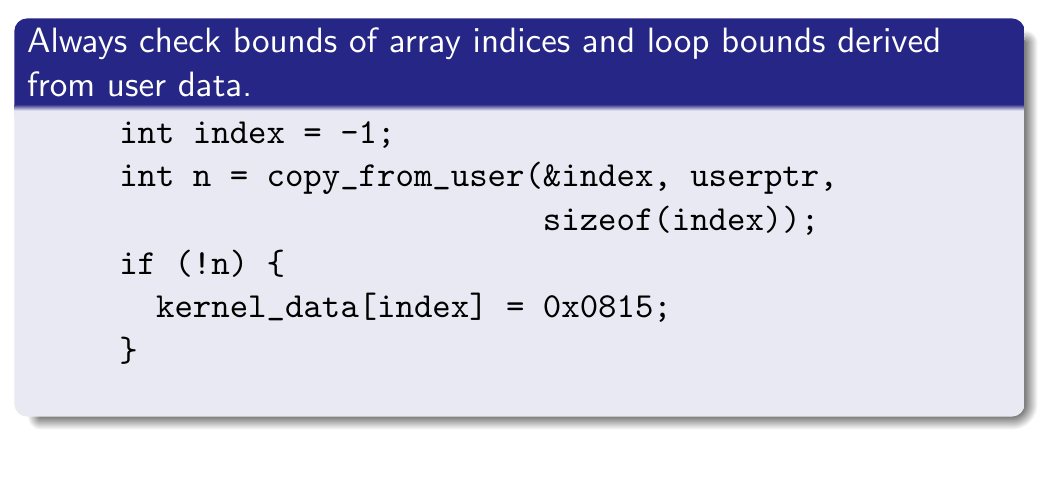
\includegraphics[width=.9\textwidth]{range-bug-sosp01}
	
\end{frame}

%-------------------------------------------------
\begin{frame}[plain]
	\frametitle{Introduction -- 9 years ago}
	\centering
	Lines of Code in Linux
	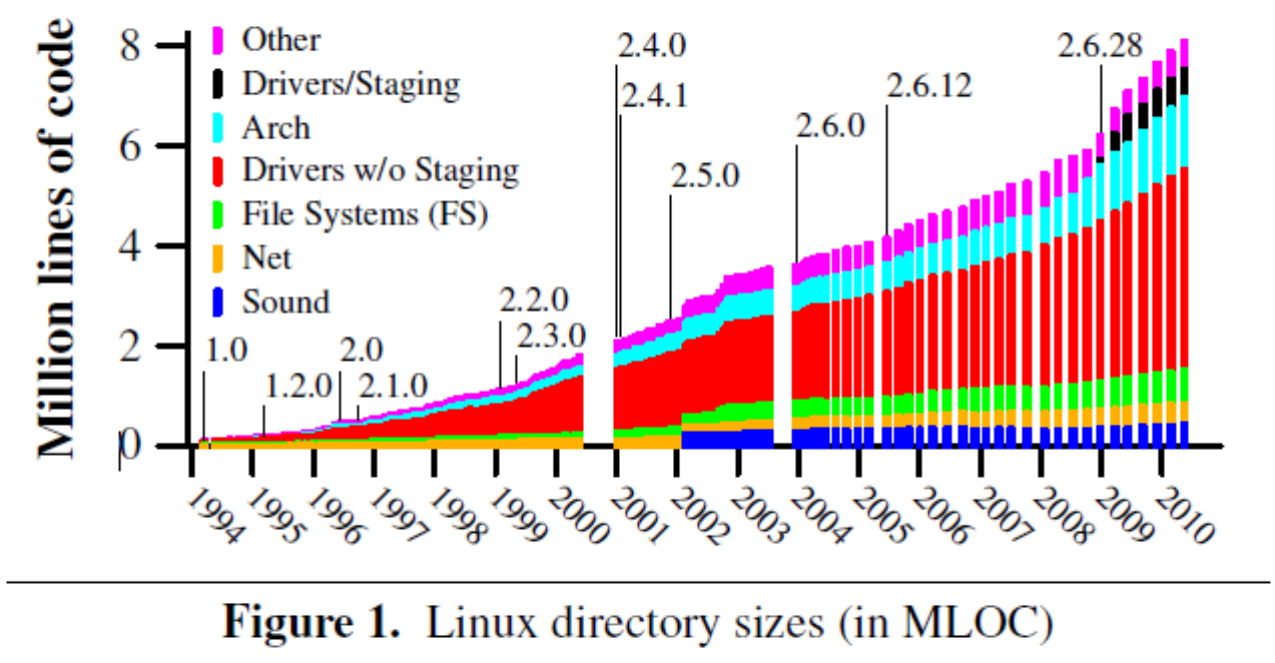
\includegraphics[width=.9\textwidth]{linux-asplos11}
	
\end{frame}


%-------------------------------------------------
\begin{frame}[plain]
	\frametitle{Introduction -- 9 years ago -- Comparative fault count}
	\centering
	
	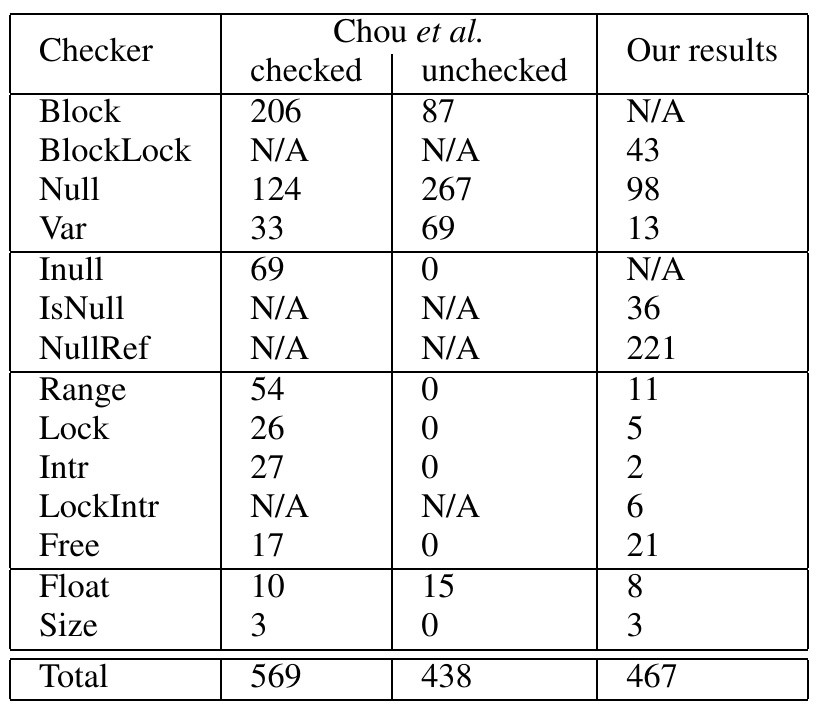
\includegraphics[width=.6\textwidth]{bug-check-asplos11}
	
\end{frame}

%-------------------------------------------------
\begin{frame}[plain]
	\frametitle{Introduction -- 9 years ago }
	\centering
	Per finding and fixing difficulty, and impact likelihood
	
	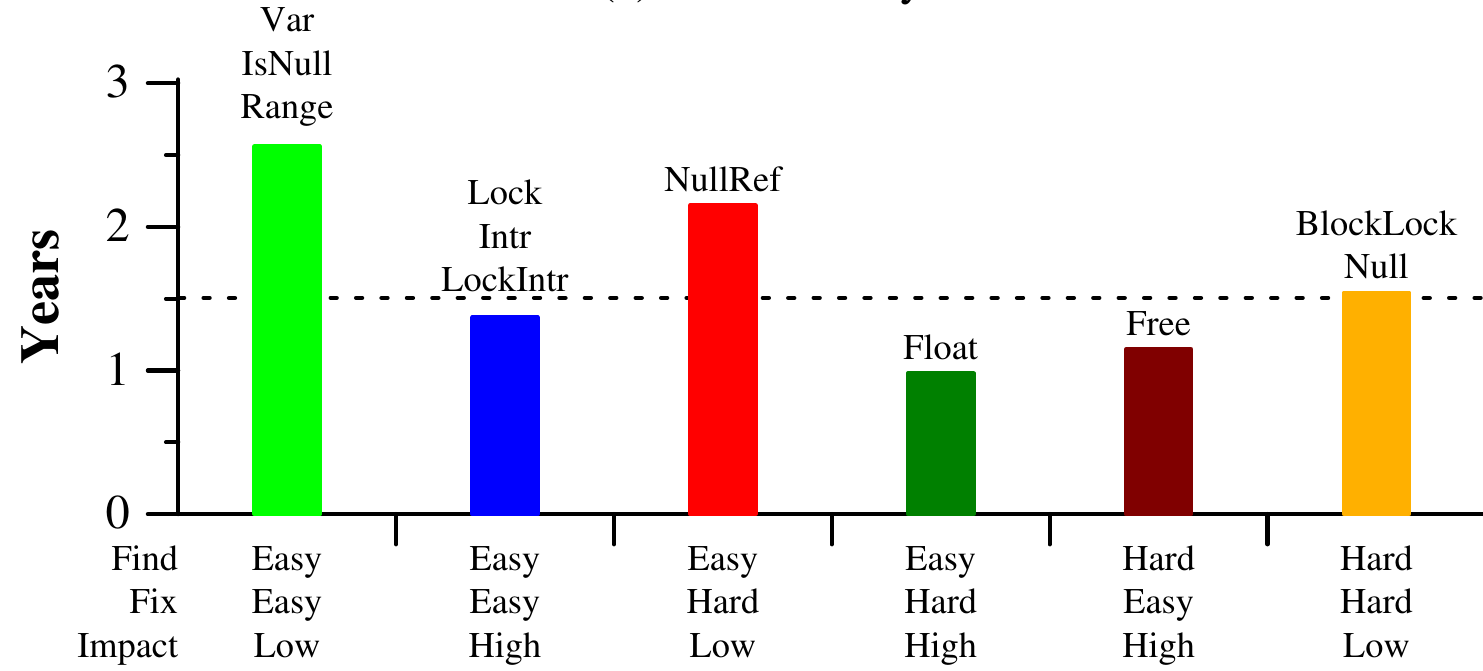
\includegraphics[width=.8\textwidth]{bug-life-asplos11}
	
\end{frame}
%-------------------------------------------------
\begin{frame}[plain]
	\frametitle{Introduction -- 9 years ago -- Linux kernel vulnerabilities}
	\centering
	141 vulnerabilities from CVE (Jan 2010 ~ Mar 2011)
	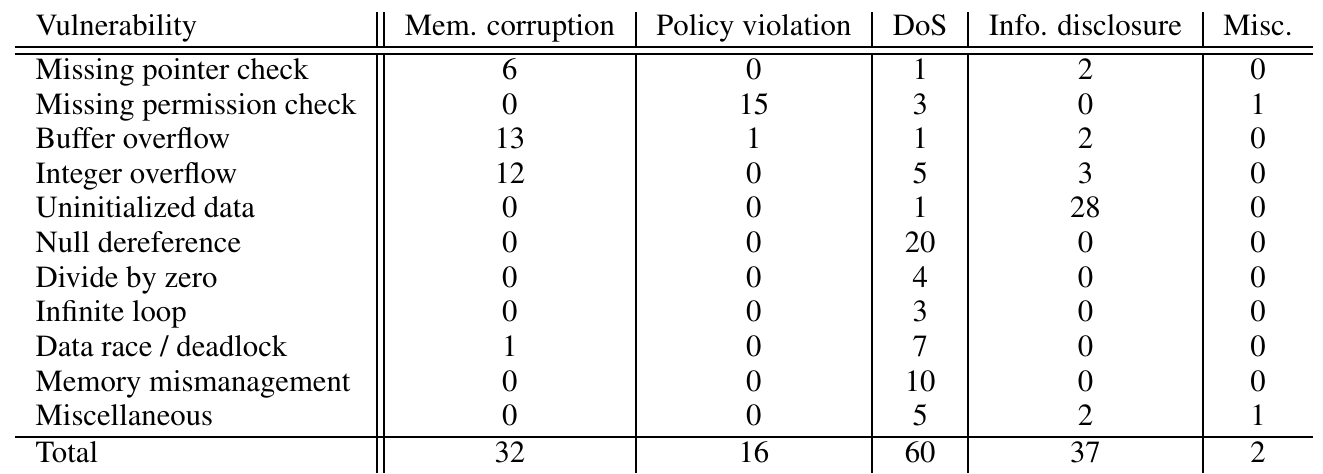
\includegraphics[width=1.\textwidth]{bugs-apsys11}
	
\end{frame}


%-------------------------------------------------
\begin{frame}[plain]
	\frametitle{Introduction -- 9 years ago -- Linux kernel vulnerabilities}
	\centering
	Distribution of 141 Vulnerabilities(Jan 2010 ~ Mar 2011)
	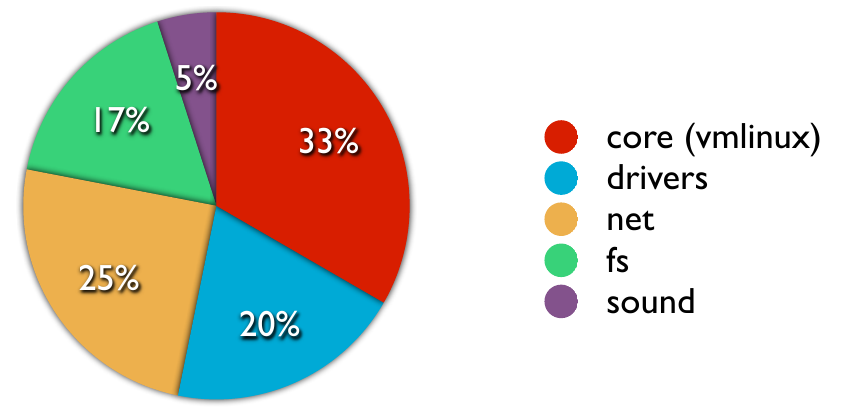
\includegraphics[width=.7\textwidth]{dist-bugs-apsys11}
	\begin{itemize}
		\item Vulnerabilities are evenly distributed in all parts of kernel
	
	\end{itemize}
\end{frame}

%-------------------------------------------------
\begin{frame}[plain]
	\frametitle{Introduction -- 9 years ago -- Linux kernel vulnerabilities}
	\centering
	 Number of vulnerabilities that existing runtime tools can prevent
	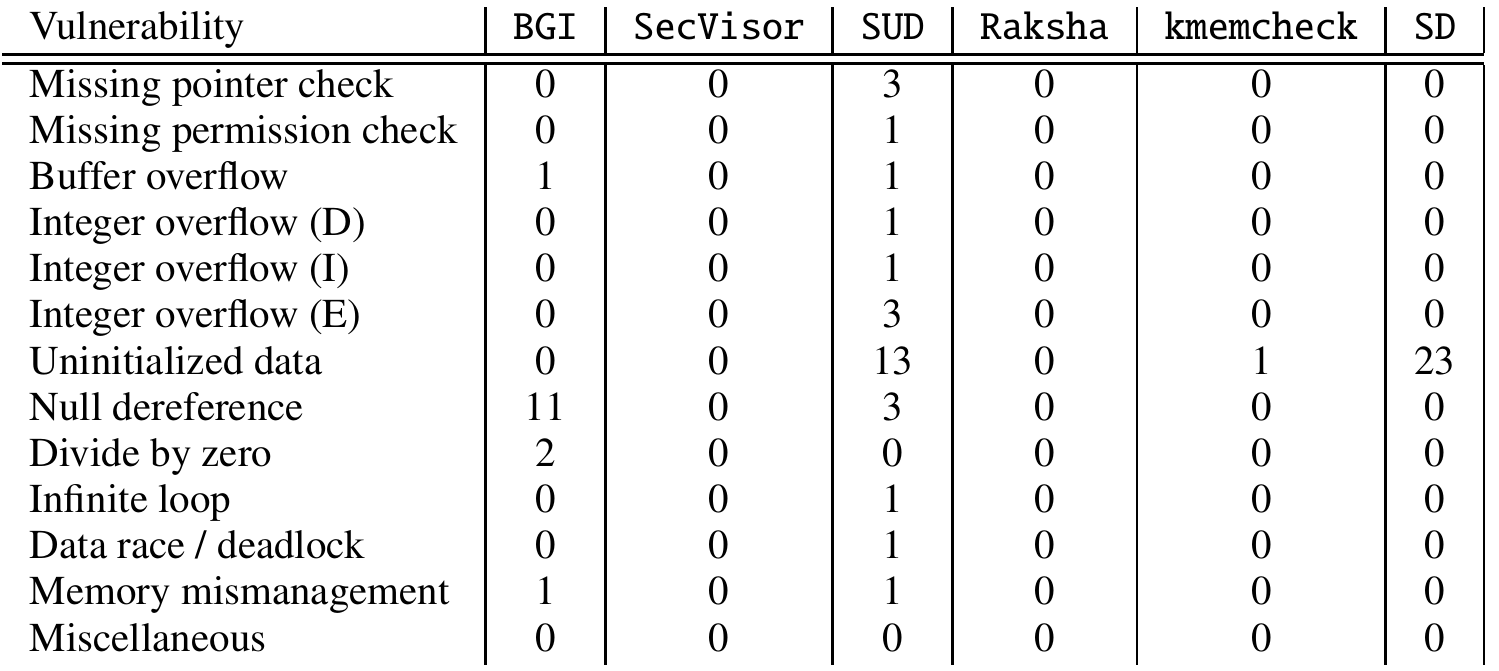
\includegraphics[width=.9\textwidth]{bug-checkers-apsys11}
	
	\begin{itemize}
	
	\item A technique that targets at only one of them is of limited use	
    \end{itemize}
\end{frame}
%-------------------------------------------------

%-------------------------------------------------
\begin{frame}[plain]
	\frametitle{References}

	\begin{itemize}
		
		\item  An empirical study of operating systems errors, SOSP 2001
		\item Linux kernel vulnerabilities: State-of-the-art defenses and open problems,APSYS 2011
		\item  Faults in linux: ten years later,ASPLOS 2011
		
	\end{itemize}
	
	
\end{frame}
%-------------------------------------------------
%-------------------------------------------------
\end{document}